\documentclass{scrartcl}
\usepackage{german}
\usepackage[T1]{fontenc}
\usepackage[utf8]{inputenc}
\usepackage[german]{babel}

% zusätzliche mathematische Symbole, AMS=American Mathematical Society
\usepackage{amssymb}
\usepackage{stmaryrd}

% fürs Einbinden von Graphiken
\usepackage{graphicx}

% für Namen etc. in Kopf- oder Fußzeile
\usepackage{fancyhdr}

% erlaubt benutzerdefinierte Kopfzeilen
\pagestyle{fancy}

% Definition der Kopfzeile
\lhead{
	\begin{tabular}{ll}
		Fisnik Zeqiri & 4306430 \\
		Felix  Karg   & 4342014
	\end{tabular}
}
\chead{}
\rhead{\today{}}
\lfoot{}
\cfoot{Seite \thepage}
\rfoot{}

\begin{document}
    \section*{Antworten zum Übungsblatt Nr. 5}

        \section*{Aufgabe 1}
            Beh.: Die kDNF ist die Kostenminimalste DNF-Darstellung. \\ \\
            Im Allgemeinen beinhaltet eine kDNF nun einen Disjunktionsterme $m*x$ sowie möglicherweise $m*x'$.
            Wenn man diese Beiden nun streicht und stattdessen nur noch $m$ innerhalb des Terms vorkommen lässt,
            beinhaltet er weniger Disjunktionsterme als die kDNF und lässt sich dadurch zwingendermaßen günstiger
            darstellen als diese. $ \lightning $


        \section*{Aufgabe 2}
        \subsection*{2 a)}
            Angenommen, ein primimplikant von $f$ enthält ein negatives Literal. Dann gibt es mindestens eine
            Belegung $b_0..b_n$ und $a_0..a_n$ mit $a < b$ bei der $f(b) < f(a)$, da ein $b_c = 1$ durch das 
            Negative Literal $0$ ist, wobei dieselbe stelle mit $a_c = 0, 1$ ist und ansonsten 
            $a_d = b_d$ gilt ($a > b$). $\lightning$

        \subsection*{2 b)}
            Die Primimplikanten des Minimalpolynoms sind insofern eindeutig bestimmt, bzw.
            Wesentlich, als dass es zwar Implikanten gibt die diese auch überdecken, allerdings
            werden diese auch von erwähnten Primimplikanten überdeckt. Insofern sind diese nur
            Wesentlich als dass es über die Bedingung (Primimplikanten) keine kürzeren gibt,
            die die jeweiligen Bereiche abdecken.

	\section*{Aufgabe 3}
	\begin{itemize}
		\item[a)] Quine-McCluskey:\\
		
	\begin{minipage}{0.3\textwidth}
	$ L_{0}^{\{x1,x2,x3,x4\}}: $\\	
			\begin{tabular}{llll}
		0 & 0 & 0 & 0\\ \hline
		0 & 0 & 0 & 1\\
		0 & 1 & 0 & 0\\
		1 & 0 & 0 & 0\\ \hline
		0 & 1 & 0 & 1\\
		0 & 1 & 1 & 0\\
		1 & 0 & 1 & 0\\
		1 & 1 & 0 & 0\\ \hline
		0 & 1 & 1 & 1\\
		1 & 1 & 1 & 0\\\hline
		1 & 1 & 1 & 1\\
					
	\end{tabular}
	\end{minipage}	
	\begin{minipage}{0.3\textwidth}	
	$ L_{1}^{\{x1,x2,x3\}}: $\\
	\begin{tabular}{llll}
		0 & 0 & 0 & -\\ \hline
		0 & 1 & 0 & -\\ \hline
		0 & 1 & 1 & -\\ \hline
		1 & 1 & 1 & -\\ 
	\end{tabular}\\\\
	$ L_{1}^{\{x1,x2,x4\}}: $\\
	\begin{tabular}{llll}
		0 & 1 & - & 0\\
		1 & 0 & - & 0\\ \hline
		0 & 1 & - & 1\\
		1 & 1 & - & 0\\ 
	\end{tabular}\\\\
	$ L_{1}^{\{x1,x3,x4\}}: $\\
	\begin{tabular}{llll}
		0 & - & 0 & 0\\ \hline
		0 & - & 0 & 1\\
		1 & - & 0 & 0\\ \hline
		1 & - & 1 & 0\\ 
	\end{tabular}\\\\
	$ L_{1}^{\{x2,x3,x4\}}: $\\
	\begin{tabular}{llll}
		- & 0 & 0 & 0\\ \hline
		- & 1 & 0 & 0\\ \hline
		- & 1 & 1 & 0\\ \hline
		- & 1 & 1 & 1\\ 
	\end{tabular}\\\\

	\end{minipage}

\begin{minipage}{0.3\textwidth}	
	$ L_{2}^{\{x1,x2\}}: $\\
	\begin{tabular}{llll}
		0 & 1 & - & -\\ \hline	
	\end{tabular}\\\\
	$ L_{2}^{\{x1,x3\}}: $\\
	\begin{tabular}{llll}
		0 & - & 0 & -\\ \hline	
	\end{tabular}\\\\
		$ L_{2}^{\{x2,x3\}}: $\\
	\begin{tabular}{llll}
		- & 1 & 1 & -\\ \hline	
	\end{tabular}\\\\
		$ L_{2}^{\{x1,x4\}}: $\\
	\begin{tabular}{llll}
		1 & - & - & 0\\ \hline	
	\end{tabular}\\\\
		$ L_{2}^{\{x2,x4\}}: $\\
	\begin{tabular}{llll}
		- & 1 & - & 0\\ \hline	
	\end{tabular}\\\\
		$ L_{2}^{\{x3,x4\}}: $\\
	\begin{tabular}{llll}
		- & - & 0 & 0\\ \hline	
	\end{tabular}\\\\
	\end{minipage}\\
	Alle $ L_{2} $ lassen sich nicht weiter kürzen und sind daher Primimplikanten.

	 \item[b)] Hypercube:\\
	 Die blauen Fächen sind die Primimplikanten\\
	 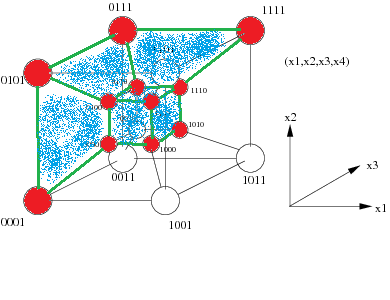
\includegraphics[width=14cm]{hypercube.png}\\

         \item[c)]
             Vollständiges Polynom:\\
             f1 = x1'x2'x3'x4'+x1'x2'x3'x4+x1'x2x3'x4'+x1x2'x3'x4'+x1'x2x3'x4+x1'x2x3x4'+x1x2'x3x4'+\\
             x1x2x3'x4'+x1'x2x3x4+x1x2x3x4'+x1x2x3x4\\
             cost1 = 11, cost2 = 48\\
         \end{itemize}

	\section*{Aufgabe 4}
	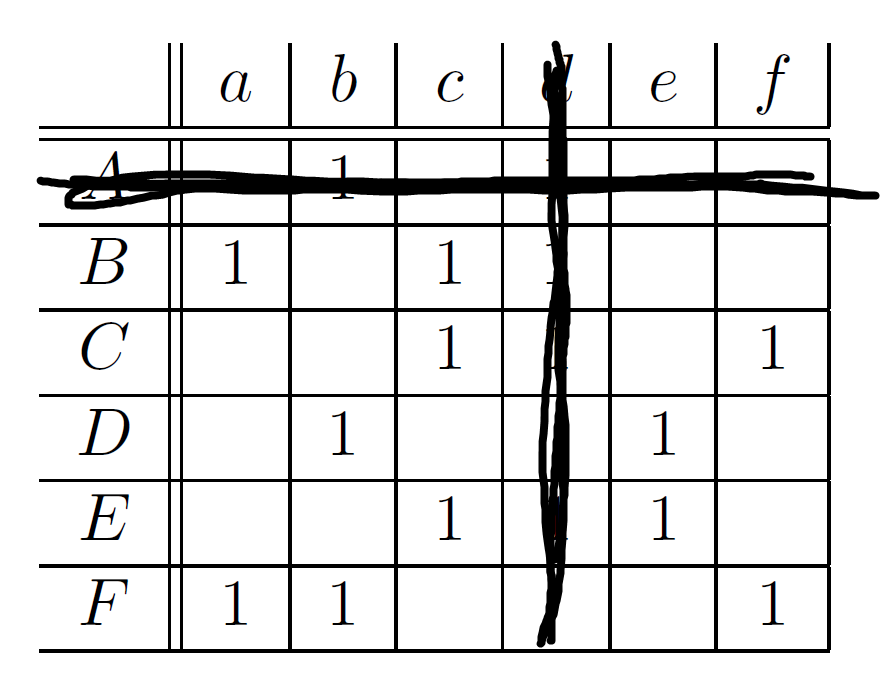
\includegraphics[width=14cm]{primtafel.png}\\
	1.) Wesentlicher Implikant: Gibt keins\\
	2.) Spaltendominanz: Spalte d) dominiert c) -> d) wird gestrichen\\
	3.) Zeilendominanz: Zeile D) dominiert A) -> A) wird gestrichen\\
	4.) Peticks Methode:\\ 
	(B+F)*(D+F)*(B+C+E)*(D+E)*(C+F) =\\
	(BD+BF+FD+F)*(BD+CD+ED+BE+CE+E)*(C+F)=\\
	(BD+BDC+BDE+BDE+BDCE+BDE+BFD+BFCD+BFED+BFE+BFCE+BFE+FDB+FDC+\\FDE+FDBE+FDCE+FDE+FBD+FCD+FED+FBE+FCE+FE)*(C+F)=\\
	(BDC+BDC+BDEC+BDEC+BDCE+BDEC+BFDC+BFCD+BFEDC+BFEC+BFCE+BFEC+\\FDBC+FDC+FDEC+FDBEC+FDCE+FDEC+FBDC+FCD+FEDC+FBEC+FCE+FEC+BDF+\\BDCF+BDEF+BDEF+BDCEF+BDEF+BFD+BFCD+BFED+BFE+BFCE+BFE+FDB+FDC+\\FDE+FDBE+FDCE+FDE+FBD+FCD+FED+FBE+FCE+\textbf{FE})\\
	=> Bei Gleichen Kosten ist FE minimal.
	
	
\end{document}
